\chapter{音频接口程序设计}
\addthumb{音频接口程序设计}{\bf 音频}{white}{gray}

\section{实验目的}
\begin{itemize}\itemsep=-3pt
  \item 了解音频编、解码的作用和工作原理;
  \item 学习 Linux 系统的音频接口编程方法.
\end{itemize}

\section{接口介绍}
	S5PV210 片内集成了音频子系统,支持多种音频编解码,包含IIS总线接口.
IIS总线通过串行方式传输数字音频、调制/解调, 实现音频输入/输出、寄存器控制和
状态信息获取等, 可与多种音频接口芯片连接.

	本实验系统使用的CODEC芯片为 WM8976.它采用~$\Delta$--$\Sigma$~转换工作原理
进行模拟/数字之间的转换.该芯片驱动程序在

  \$(KERNELPATH)/drivers/sound/soc/codecs/wm8976.c

\section{原理概述}
	内核编译时需要有声音支持.

\subsection{OSS}
	Linux 系统的音频驱动主要有两类: OSS(Open Sound System)和 ALSA(Advanced
Linux Sound Architecture).其中 OSS 主要出现在早期的 Linux版本中.
与 OSS 相关的设备节点主要有两个:

\begin{itemize}\itemsep=-3pt
  \item /dev/dsp(主设备号14,次设备号3),负责音频数据的输入~(A/D~转换)和输出
		~(D/A~转换)、工作方式设置(采样/输出频率、通道数、数据格式等等);
  \item /dev/mixer(主设备号14,次设备号0),混音及音量设置、高低音等等.
\end{itemize}

	请参考\$(KERNEL\_PATH)/include/linux/soundcard.h~中的说明完成音频接口设置.
(如,设置双声道, channels=2; ioctl(fd, SNDCTL\_DSP\_CHANNELS, \&channels);)
编写应用程序,实现简单的录音和放音.记录模拟/数字音频转换结果.

	通过 /dev/dsp(或/dev/audio,主设备号13,次设备号4)设置给定的采样/输出
模式.常用的设置命令有:
\begin{itemize}\itemsep=-3pt
  \item SNDCTL\_DSP\_RESET
  \item SNDCTL\_DSP\_SPEED,采样/输出率,如8000Hz、44100Hz、48000Hz等.
		$\Delta-\Sigma$转换器通过晶振的有限个分频得到采样率,因此不能 直接
        实现任意频率的采样/输出.
  \item SNDCTL\_DSP\_SAMPLESIZE,采样值的数据位大小.
  \item SNDCTL\_DSP\_CHANNELS,通道数,mono(1)或stereo(2).
  \item SOUND\_PCM\_WRITE\_CHANNELS,输出通道数,通常和输入通道数一致.
  \item SNDCTL\_DSP\_SETFRAGMENT,缓冲数据块大小.
  \item SNDCTL\_DSP\_SETFMT、SNDCT\_DSP\_GETFMTS,设置/获取数据格式.这些格式
		包括~$\mu$--律~(AFMT\_MU\_LAW)、~A--律~(AFMT\_A\_LAW)、~无符号8位~
		(AFMT\_U8)、~带符号8位(AFMT\_S8)、~16位大端或小端模式~(AFMT\_S16\_LE、
		~AFMT\_U16\_BE)等等.
\end{itemize}

	对混音器(/dev/mixer)的常用命令有:
\begin{itemize}\itemsep=-3pt
  \item SOUND\_MIXER\_NRDEVICES,获取设备数量.
  \item SOUND\_MIXER\_VOLUME,总音量设置.音量取值范围是0$\sim$100.
  \item SOUND\_MIXER\_BASS、SOUND\_MIXER\_TREBLE,低音、高音设置.
  \item ~SOUND\_MIXER\_PCM、~SOUND\_MIXER\_LINE、~SOUND\_MIXER\_MIC~等,对
		各音源音量的独立设置. 
  \item SOUND\_MIXER\_IGAIN,输入增益.
  \item SOUND\_MIXER\_OGAIN,输出增益.
\end{itemize}

\subsection{ALSA}
	现在的Linux发行版更多的采用ALSA音频驱动.与OSS不同的是, ALSA应用程序
通过ALSA API完成对设备的操作,不再使用 open,close,ioctl,read,write 等低级
系统调用.因此 ALSA 应用程序中看不到设备文件,有的只是对ALSA 函数的调用.
编译ALSA程序需要链接 asound 库.

	下面是一些API的例子:

\lstset{language=c}
%\lstset{backgroundcolor=\color{bg}}
\begin{lstlisting}{}
  /* Allocate the snd_pcm_hw_params_t structure on the stack. */
  snd_pcm_hw_params_t *hwparams;
  snd_pcm_hw_params_alloca(&hwparams);
  
  /* 打开 PCM 设备 */
  char *pcm_name = "plughw:0,0";
  snd_pcm_open(&pcm_handle, pcm_name, SND_PCM_STREAM_PLAYBACK, 0);
  
  /* 初始化 PCM 参数*/
  snd_pcm_hw_params_any(pcm_handle, hwparams);
  
  /* PCM 命令集的形式是
  	snd_pcm_hw_params_can_<capability>
  	snd_pcm_hw_params_is_<property>
  	snd_pcm_hw_params_get_<parameter>
   - 一些重要的参数,包括缓冲区大小、通道数、采样格式、速率等,可以通过
  	snd_pcm_hw_params_set_<parameter> 调用实现 */
  
  /* 设置数据格式:16bit-signed-little-endian */
  snd_pcm_hw_params_set_format(pcm_handle, hwparams,
         SND_PCM_FORMAT_S16_LE);
  
  /* stereo */ 
  snd_pcm_hw_params_set_channels(pcm_handle, hwparams, 2);
  
  /* 设置采样率 44.1kHz */
  snd_pcm_hw_params_set_rate(pcm_handle, hwparams, 44100, 0);
  
  /* 将数据写入设备 (Digital to Analogue) , 函数返回实际写入的帧数 */
  snd_pcm_write(pcm_handle, buffer, num_of_frames);
  
  /* 对混音器操作,通过 snd_mixer_<parameter/property> 一组指令完成 */
\end{lstlisting}


\section{实验内容}

	根据内核配置,选择适当的音频驱动,实现数字音频的采集与回放.

\section{实验报告要求}
\begin{itemize}\itemsep=-3pt
  \item 将实验采集的数据与信号源产生的实际信号对比,将输出的预期信号与示波器
		测量到的信号对比,分析产生差异的原因;
  \item 思考:如果在信号采集过程中还包含了数据处理工作,如何保证信号的连续性?
\end{itemize}

% **************************************************
\newpage
\tt [附] $\Delta-\Sigma$ AD转换器原理

Delta-Sigma ($\Delta-\Sigma$) ADC

One of the more advanced ADC technologies is the so-called delta-sigma,
or $\Delta-\Sigma$ (using the proper Greek letter notation). In mathematics
and physics, the capital Greek letter delta ($\Delta$) represents difference
or change, while the capital letter sigma ($\Sigma$) represents summation:
the adding of multiple terms together. Sometimes this converter is referred
to by the same Greek letters in reverse order: sigma-delta, or $\Sigma-\Delta$.

In a $\Sigma-\Delta$ converter, the analog input voltage signal is connected
to the input of an integrator, producing a voltage rate-of-change, or slope,
at the output corresponding to input magnitude. This ramping voltage is then
compared against ground potential (0 volts) by a comparator. The comparator
acts as a sort of 1-bit ADC, producing 1 bit of output ("high" or "low")
depending on whether the integrator output is positive or negative. The
comparator's output is then latched through a D-type flip-flop clocked at a
high frequency, and fed back to another input channel on the integrator,
to drive the integrator in the direction of a 0 volt output. The basic
circuit looks like this:

\begin{figure}[!h]
\centering
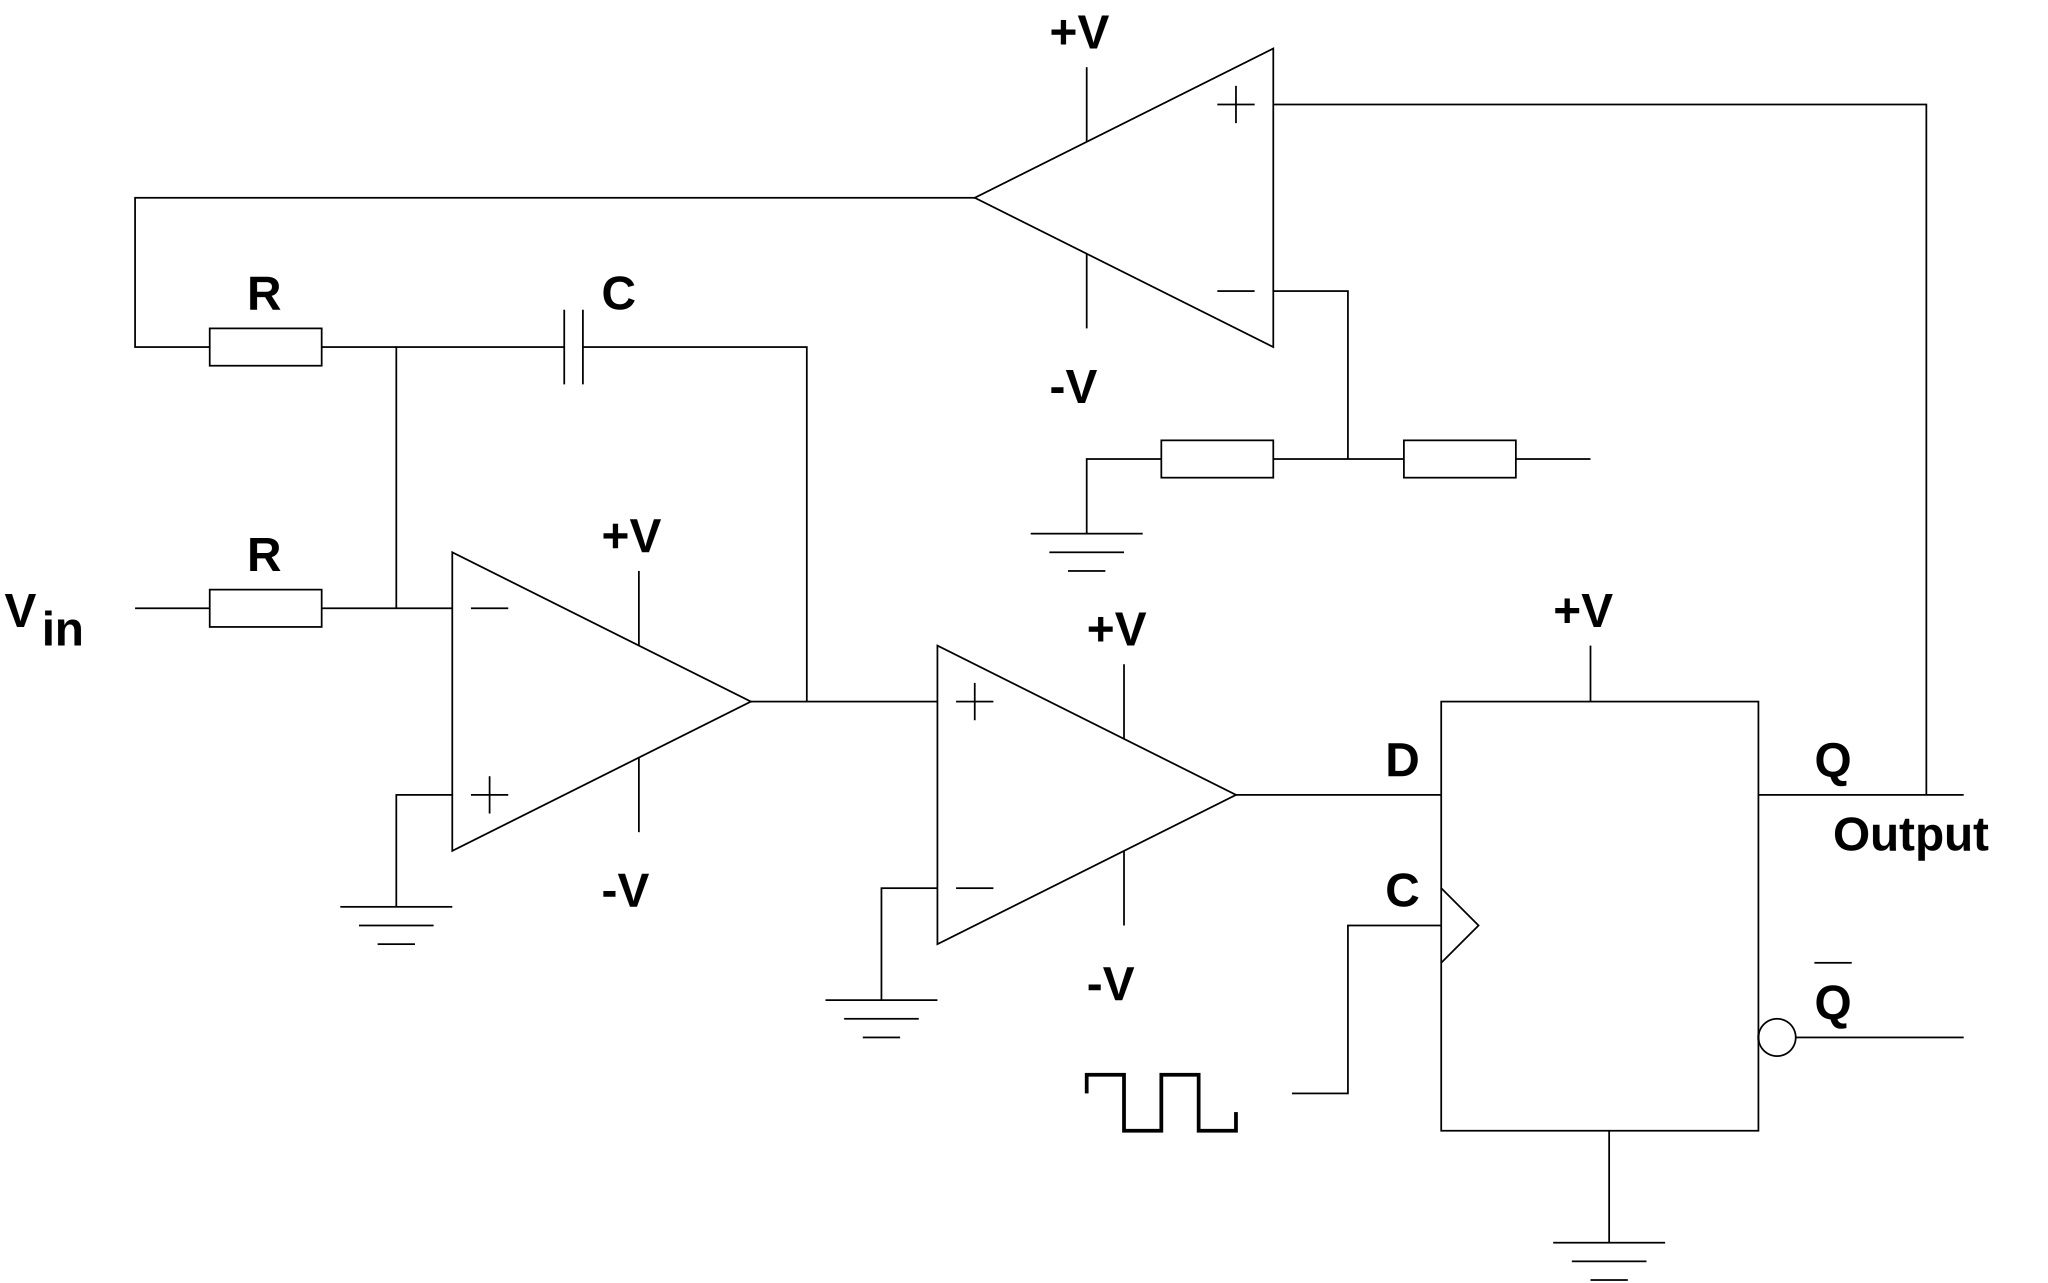
\includegraphics[width=0.6\textwidth]{adc1}
\end{figure}

The leftmost op-amp is the (summing) integrator. The next op-amp the
integrator feeds into is the comparator, or 1-bit ADC. Next comes the
D-type flip-flop, which latches the comparator's output at every clock
pulse, sending either a "high" or "low" signal to the next comparator at
the top of the circuit. This final comparator is necessary to convert the
single-polarity 0V/5V logic level output voltage of the flip-flop into a
+V/-V voltage signal to be fed back to the integrator.If the integrator
output is positive, the first comparator will output a "high" signal to the D
input of the flip-flop. At the next clock pulse, this "high" signal will be
output from the Q line into the noninverting input of the last comparator.
This last comparator, seeing an input voltage greater than the threshold
voltage of 1/2 +V, saturates in a positive direction, sending a full +V
signal to the other input of the integrator. This +V feedback signal tends
to drive the integrator output in a negative direction. If that output
voltage ever becomes negative, the feedback loop will send a corrective
signal (-V) back around to the top input of the integrator to drive it in
a positive direction. This is the delta-sigma concept in action: the first
comparator senses a difference ($\Delta$) between the integrator output and
zero volts. The integrator sums ($\Sigma$) the comparator's output with the
analog input signal. Functionally, this results in a serial stream of bits
output by the flip-flop. If the analog input is zero volts, the integrator
will have no tendency to ramp either positive or negative, except in
response to the feedback voltage. In this scenario, the flip-flop output
will continually oscillate between "high" and "low," as the feedback system
"hunts" back and forth, trying to maintain the integrator output at zero
volts: 
 
\begin{figure}[!h]
\centering
$\Delta\Sigma$ converter operation with\\ 0 volt analog input\\
\includegraphics[width=.5\textwidth]{wave1}
\end{figure}

If, however, we apply a negative analog input voltage, the integrator will
have a tendency to ramp its output in a positive direction. Feedback can
only add to the integrator's ramping by a fixed voltage over a fixed time,
and so the bit stream output by the flip-flop will not be quite the same: 

\begin{figure}[!h]
\centering
$\Delta\Sigma$ converter operation with\\ small negative analog input\\
\includegraphics[width=.5\textwidth]{wave2}
\end{figure}

By applying a larger (negative) analog input signal to the integrator,
we force its output to ramp more steeply in the positive direction. Thus,
the feedback system has to output more 1's than before to bring the
integrator output back to zero volts: 

\begin{figure}[!h]
\centering
$\Delta\Sigma$ converter operation with\\ medium negative analog input\\
\includegraphics[width=.5\textwidth]{wave3}
\end{figure}

As the analog input signal increases in magnitude, so does the occurrence
of 1's in the digital output of the flip-flop: 

\begin{figure}[!h]
\centering
$\Delta\Sigma$ converter operation with\\ large negative analog input\\
\includegraphics[width=.5\textwidth]{wave4}
\end{figure}

A parallel binary number output is obtained from this circuit by averaging
the serial stream of bits together. For example, a counter circuit could be
designed to collect the total number of 1's output by the flip-flop in a
given number of clock pulses. This count would then be indicative of the
analog input voltage. Variations on this theme exist, employing multiple
integrator stages and/or comparator circuits outputting more than 1 bit,
but one concept common to all $\Delta-\Sigma$ converters is that of
oversampling. Oversampling is when multiple samples of an analog signal are
taken by an ADC (in this case, a 1-bit ADC), and those digitized samples are
averaged. The end result is an effective increase in the number of bits
resolved from the signal. In other words, an oversampled 1-bit ADC can do
the same job as an 8-bit ADC with one-time sampling, albeit at a slower rate. 
% *****************************************************************
\rm
